\chapter{Methodology}
\label{chap:methodology}
% Target ~9 pages. Rubric criterion: "awareness and critical evaluation
% of alternatives" -- see Section 3.6.

\section{Working Theory: Evaluative Epistemic Filtering}
\label{sec:working-theory}

The framework developed in this chapter rests on a working theory of
why LLM evaluators systematically under-score culturally unfamiliar
writing. This section states that theory precisely, identifies the
conditions that sustain the phenomenon, and derives the observable
signatures that the experiments in Chapter~4 test.

\begin{definition}[Evaluative epistemic filtering]
\label{def:eef}
Let $E$ be an essay, $f_{\mathrm{human}}(E)$ the score assigned by a
trained human examiner under a rubric $R$, and
$f_{\mathrm{LLM}}(E \mid \theta)$ the score assigned by an LLM
evaluator whose parameters $\theta$ were estimated from a training
distribution $\mathcal{D}$. Evaluative epistemic filtering occurs when
\begin{equation}
\label{eq:eef}
\mathbb{E}\!\left[\, f_{\mathrm{LLM}}(E \mid \theta_{\mathcal{D}})
  - f_{\mathrm{human}}(E) \,\middle|\, c(E) \right] \neq 0,
\end{equation}
where $c(E)$ denotes the rhetorical tradition of the essay, and the
deviation is systematic in $c$: essays whose rhetorical form is
under-represented in $\mathcal{D}$ receive systematically deflated
scores relative to human judgment, independent of argumentative merit.
\end{definition}

The definition makes two commitments. First, the filter is a property
of the \emph{evaluator}, not of the essay: the same essay receives
different treatment under evaluators with different training
distributions. Second, the deviation is conditional on rhetorical
tradition rather than on language proficiency; this is what
distinguishes evaluative epistemic filtering from the legitimate
scoring of weaker English, and what the matched-cohort experimental
design in Section~\ref{sec:experimental-design} is built to isolate.

Four conditions jointly sustain the filter in current systems. First,
training corpora over-represent WEIRD cultural contexts, and models
demonstrably absorb the corresponding value orientation
\citep{tao2024cultural}. Second, the standards LLM evaluators apply
are opaque: unlike feature-based AES, where population-specific
predictors could be inspected directly \citep{vajjala2018automated},
an LLM's evaluative prior is distributed across its parameters
\citep{gallegos2024bias}. Third, diagnostic effort has concentrated on
generative outputs; the bias categories formalised by
\citet{dorleon2026uncovering} have no evaluative counterpart in the
literature. Fourth, the observable symptom (L1-linked scoring
disparities) is now documented \citep{gayed2026firstlanguage} but has
not been connected to a mitigation mechanism.

The theory yields three testable signatures, which map directly onto
the hypotheses of Chapter~1. First, a systematic scoring gap should
appear between rhetorical-tradition cohorts matched on human-rated
quality (H1). Second, the gap should shrink when the single evaluator
is replaced by a panel whose members embody different rubric
interpretations, because their individual filters are partially
decorrelated (H2). Third, panel members should disagree measurably on
precisely the essays where filtering operates, which makes divergence
itself a detection signal (H3).
The fairness--accuracy boundary (H4) follows from the consensus
mechanism and is derived in Section~\ref{sec:camps-framework}.

\section{The CAMPS Framework}
\label{sec:camps-framework}

CAMPS (Culturally-Aware Multi-Perspective Scoring) operationalises a
single design principle: if no evaluator judges from nowhere
(Section~\ref{sec:theory}), then fairness is pursued through a
\emph{plurality} of explicitly declared perspectives rather than
through a pretended neutrality. Concretely, the plurality is the panel
of five cultural rubric interpretations specified in
Section~\ref{sec:scaling-panel} (Western, Southeast Asian, East
Asian, Mekong/Vietnamese, and a neutral regulatory ideal; see
Table~\ref{tab:lens-panel}), each declared in an inspectable system
prompt rather than hidden in model weights, continuing the
multi-perspective principle introduced in
Section~\ref{sec:theory}. The framework operates entirely at
inference time, requires no model retraining or weight access, and
treats every underlying LLM as a black box reachable through an API.
Figure~\ref{fig:camps-architecture} shows the pipeline; the five
components are specified below.

\begin{figure}[htbp]
\centering
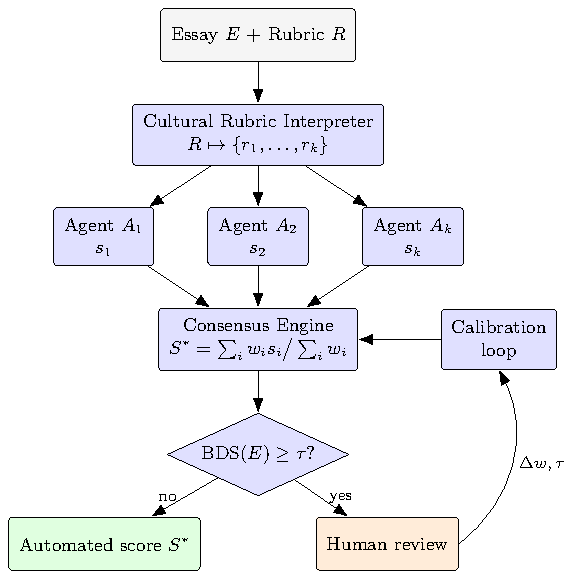
\includegraphics[width=0.72\textwidth]{figures/fig-camps-architecture}
\caption[The CAMPS pipeline]{The CAMPS pipeline. Each essay is scored
in parallel by $k$ \emph{culturally-calibrated} agents: LLM evaluators
whose system prompts embed a documented cultural interpretation of the
scoring rubric (Component~1). The consensus engine aggregates the
scores. The Bias Divergence Score routes contested essays to human
review, whose outcomes feed the calibration loop. CAMPS components are
shaded blue; inputs and outcomes are unshaded.}
\label{fig:camps-architecture}
\end{figure}

\subsection*{Component 1: Cultural Rubric Interpreter (CRI)}
Given the scoring rubric $R$, the CRI produces $k$ culturally-adapted
interpretations $\{r_1, \dots, r_k\}$ through system-level prompting.
Each interpretation is grounded in the contrastive-rhetoric literature
reviewed in Section~\ref{sec:lit-rhetoric} rather than in improvised
personas. The Southeast Asian interpretation, for example, instructs
the agent to recognise inductive thesis development and
reader-responsible coherence \citep{hinds1987reader} as valid
realisations of the rubric's coherence criterion. The neutral
interpretation is retained as a regulatory ideal in Fricker's sense
\citep{fricker2007epistemic}, not as an achievable standpoint.
The full prompt texts are reproduced verbatim in
Appendix~\ref{chap:appendix-prompts}.

\subsection*{Component 2: Evaluator agent pool}
Each interpretation is bound to an independent evaluator agent, and
each agent scores the essay without access to the other agents'
outputs:
\begin{equation}
s_i = A_i(E, r_i), \qquad i = 1, \dots, k,
\end{equation}
with temperature fixed at $t = 0.0$ and structured (JSON) output, so
that every run is deterministic and reproducible. Independence at this
stage is deliberate: the MALIBU results \citep{mirza2025malibu} caution
that interacting agents can amplify rather than cancel bias, so CAMPS
confines interaction to the aggregation stage, where it is
mathematically controlled.

\subsection*{Component 3: Consensus aggregation}
The panel's scores are combined as a weighted mean,
\begin{equation}
\label{eq:consensus}
S^{*}(E) = \frac{\sum_{i=1}^{k} w_i\, s_i(E)}{\sum_{i=1}^{k} w_i},
\qquad w_i \geq 0,
\end{equation}
with weights initialised equal. Because $S^{*}$ is linear in the
agents' scores, any reweighting that raises the expected score of one
cohort must lower another's whenever the agents disagree
systematically; this is the mechanism behind the fairness--accuracy
boundary hypothesised in H4, and Section~\ref{sec:experimental-design}
describes how the weight space is swept to locate it empirically.

\subsection*{Component 4: Bias Divergence Score (BDS)}
The framework's detection signal is the dispersion of the panel:
\begin{equation}
\label{eq:bds}
\mathrm{BDS}(E) = \sqrt{\frac{1}{k} \sum_{i=1}^{k}
  \bigl(s_i(E) - S^{*}(E)\bigr)^{2}}.
\end{equation}
A low BDS means the cultural interpretations converge: the essay is
scored the same way regardless of the lens, and the automated score can
be trusted. A high BDS means the lenses disagree, which under the
working theory is exactly the signature of an essay whose score depends
on culturally contingent expectations; such essays are flagged for
human review. The pilot fixed the threshold at $\tau = 0.75$ on the
operational argument that 0.75 standard deviations corresponds to a
two-band disagreement under IELTS-style scoring. Part~B replaces this
hand-set value with a threshold calibrated by receiver operating
characteristic analysis against multi-rater human ground truth (H3),
as specified in Section~\ref{sec:experimental-design}.

\subsection*{Component 5: Calibration loop}
Outcomes of human review feed back into the framework in two ways: the
consensus weights $w_i$ are re-optimised to maximise agreement with
human scores subject to a cohort-fairness constraint, and the
threshold $\tau$ is re-estimated as review outcomes accumulate. The
loop closes the system without touching model weights; everything
learned lives in $w$ and $\tau$.

\medskip
The five components divide the framework's labour: the first two
create and apply the plurality of perspectives, the third converts
plurality into a single defensible score, and the last two turn
residual disagreement into detection and adaptation. No component
alone mitigates the filter; the fairness properties of CAMPS are a
property of the assembly.
Table~\ref{tab:framework-comparison} positions CAMPS against the
frameworks reviewed in Chapter~2 along the five capabilities the
design combines.

\begin{table}[htbp]
\centering
\caption[Capability comparison of related frameworks]{Capability
comparison. \emph{Inf.} = inference-time only; \emph{Cult.} = explicit
cultural perspectives; \emph{Eval.} = evaluative (scoring) task;
\emph{Div.} = divergence-based detection; \emph{HITL} = calibrated
human-in-the-loop trigger.}
\label{tab:framework-comparison}
\begin{tabular}{lccccc}
\hline
Framework & Inf. & Cult. & Eval. & Div. & HITL \\
\hline
CultureLLM \citep{li2024culturellm} & $\times$ & \checkmark & $\times$ & $\times$ & $\times$ \\
BiasFilter \citep{cheng2025biasfilter} & \checkmark & $\times$ & $\times$ & $\times$ & $\times$ \\
CAFES \citep{su2025cafes} & \checkmark & $\times$ & \checkmark & $\times$ & $\times$ \\
RES \citep{jang2025roundtable} & \checkmark & $\times$ & \checkmark & $\times$ & $\times$ \\
PoLL \citep{verga2024replacing} & \checkmark & $\times$ & \checkmark & $\times$ & $\times$ \\
MACD \citep{tan2026macd} & \checkmark & \checkmark & $\times$ & $\times$ & $\times$ \\
Dorleon \& Shujaa \citeyearpar{dorleon2026uncovering} & \checkmark & \checkmark & $\times$ & $\times$ & $\times$ \\
\textbf{CAMPS (this thesis)} & \checkmark & \checkmark & \checkmark & \checkmark & \checkmark \\
\hline
\end{tabular}
\end{table}

Relative to the Part~A pilot, the framework specified here differs in
three respects, each developed in the following sections: the panel is
scaled from three to five cultural interpretations with a
meta-adjudicator (Section~\ref{sec:scaling-panel}), the corpus and
cohort design are rebuilt on data that supports the comparison
(Section~\ref{sec:data}), and both the consensus weights and the BDS
threshold are calibrated empirically rather than hand-set
(Section~\ref{sec:experimental-design}).

\section{Scaling the Panel: from Three to Five Agents}
\label{sec:scaling-panel}

The pilot panel comprised three rubric interpretations: Western,
Southeast Asian, and a neutral interpretation retained as a regulatory
ideal (Section~\ref{sec:camps-framework}). Scaling to five requires a
principled answer to the question \emph{which} cultural lenses to add.
Three selection criteria are applied. A candidate lens must be
(i)~\emph{documented}: its rhetorical conventions must be described in
the contrastive-rhetoric literature, so that the CRI prompt encodes
scholarship rather than stereotype; (ii)~\emph{validatable}: the
corpus must contain a writer cohort from the corresponding tradition,
so that the lens's behaviour can be checked against real essays; and
(iii)~\emph{distinct}: the lens must be expected to diverge from the
existing panel on identifiable essay features, otherwise it adds cost
without information.

Applying these criteria to the available data
(Section~\ref{sec:data}) selects an \emph{East Asian} lens, grounded
in the reader-responsible coherence tradition documented for Japanese
and related academic writing cultures \citep{hinds1987reader} and
validatable against ICNALE's China, Japan, Korea, and Taiwan cohorts,
and a \emph{Mekong/Vietnamese} lens, motivated by the region this
research serves and validatable against the ICNALE~WEP cohorts from
Vietnam, Cambodia, Laos, and Myanmar. A Middle Eastern lens, although
well documented in the contrastive-rhetoric literature, fails the
validatable criterion for the primary corpus and is deferred to future
work. Table~\ref{tab:lens-panel} summarises the resulting panel.

\begin{table}[htbp]
\centering
\caption[The five-lens CAMPS panel]{The five-lens panel: rhetorical
grounding and the corpus cohort against which each lens's behaviour
can be validated.}
\label{tab:lens-panel}
\small
\begin{tabular}{p{2.9cm} p{5.6cm} p{3.6cm}}
\hline
Lens & Rhetorical grounding & Validating cohort \\
\hline
CRI\textsubscript{Western} & Writer-responsible coherence; explicit
thesis-first linear development \citep{kaplan1966cultural,
connor2011intercultural} & ICNALE ENS \\[3pt]
CRI\textsubscript{SEA} & Inductive, context-first development;
collectivist framing \citep{connor2011intercultural,
ishikawa2023icnale} & ICNALE THA, IDN, PHL \\[3pt]
CRI\textsubscript{EastAsian} & Reader-responsible coherence; delayed
thesis; \emph{ki-sho-ten-ketsu}-style organisation
\citep{hinds1987reader} & ICNALE CHN, JPN, KOR, TWN \\[3pt]
CRI\textsubscript{Mekong} & Proverb- and narrative-anchored
argumentation observed in Mekong-region learner writing
\citep{ishikawa2023icnale, shujaa2026llms} & ICNALE WEP VNM, KHM,
LAO, MMR \\[3pt]
CRI\textsubscript{Neutral} & Regulatory ideal: argumentative merit
irrespective of structural ordering \citep{fricker2007epistemic} &
(all cohorts) \\
\hline
\end{tabular}
\end{table}

The second architectural addition is a \emph{meta-adjudicator}: a
further LLM instance that receives the five agents' scores and their
short written rationales, and produces a reasoned consensus score,
\begin{equation}
S^{\mathrm{adj}}(E) = M\bigl(s_1, \rho_1, \dots, s_k, \rho_k\bigr),
\end{equation}
where $\rho_i$ is agent $i$'s rationale. The adjudicator is blind to the writer's identity and cohort
metadata, and runs at $t = 0.0$ like the agents. It constitutes an
alternative aggregation path to the weighted mean of
Equation~\ref{eq:consensus}. Where the weighted mean treats every
agent's judgment as exchangeable evidence, the adjudicator can weigh
\emph{arguments}, for example discounting an agent whose rationale
misidentifies the essay's structure. Experiment
E2 compares the two paths directly, and the BDS of
Equation~\ref{eq:bds} is computed from the raw agent scores in both
conditions, so the detection signal is unaffected by the choice of
aggregator. This design responds to the caution from multi-agent bias
research \citep{mirza2025malibu}: the adjudicator adds deliberation
\emph{after} independent judgment, rather than allowing agents to
influence one another during scoring.

\section{Data}
\label{sec:data}

\subsection*{Corpus selection}
The experimental design requires a corpus with four properties: essays
by Southeast Asian learners identified by first language or country;
a native-English reference cohort writing under identical task
conditions; a human-assigned quality or proficiency measure; and terms
of use permitting research at this scale. A systematic search of the
major public learner corpora found exactly one corpus satisfying all
four. TOEFL11 \citep{blanchard2013toefl11}, used in the pilot phase,
contains 12{,}100 essays across eleven first languages but includes
no Southeast Asian L1 and, by construction, no native-English cohort,
and its proficiency labels are coarse (low, medium, high). ICLE~v3
covers twenty-five L1 backgrounds without Thai or another Southeast
Asian L1; ELLIPSE offers approximately 9{,}000 human-scored learner
essays without L1 labels; EFCAMDAT records nationality and CEFR level
but has no native reference cohort.\footnote{Corpus contents verified
against their official distribution pages in July 2026: TOEFL11 via
the Linguistic Data Consortium (LDC2014T06), ICLE via UCLouvain,
ELLIPSE via its public repository, EFCAMDAT via the EF--Cambridge
Open Language Database.} The ICNALE corpus family
\citep{ishikawa2023icnale} satisfies all four properties and is
therefore adopted.

\subsection*{The ICNALE corpus family}
ICNALE (the International Corpus Network of Asian Learners of
English) collects topic-controlled English essays and speeches from
college students across ten Asian countries and regions together with
a native-English-speaker reference cohort writing under identical
conditions. Three modules are used in this thesis
(Table~\ref{tab:icnale-modules}). Critically for the present design,
every written essay addresses the same two prompts (whether college
students should hold a part-time job, and whether smoking should be
banned in restaurants), under controlled length and time conditions;
this removes the prompt-variation confound present in TOEFL11's
eight-topic design. All learner participants are placed into
CEFR-linked proficiency bands (A2, B1\_1, B1\_2, B2+) on the basis of
standardised test scores or a vocabulary-size test, which enables
proficiency-matched cohort construction.

\begin{table}[htbp]
\centering
\caption[ICNALE modules used in this thesis]{ICNALE modules used in
this thesis (contents as published on the official ICNALE
distribution site, March 2026).}
\label{tab:icnale-modules}
\small
\begin{tabular}{p{3.2cm} p{4.6cm} p{4.6cm}}
\hline
Module & Contents & Role in this thesis \\
\hline
Written Essays (WE) v2.6 & 5{,}600 essays, 200--300 words, two
controlled topics; ten Asian countries/regions plus native ENS cohort
& Primary cohorts: SEA learners and native reference \\[3pt]
Written Essays Plus (WEP) v0.7 & 2{,}340 essays from additional
countries including Vietnam, Cambodia, Laos, Myanmar & Mekong cohort;
validation of CRI\textsubscript{Mekong} \\[3pt]
Global Rating Archives (GRA) v2.1 & 140 essays, each rated by 80
raters of varied L1 and occupational backgrounds (22{,}400 ratings)
& Multi-rater human ground truth for BDS validation (E3) \\
\hline
\end{tabular}
\end{table}

\subsection*{Cohort construction and sampling}
Figure~\ref{fig:sampling-flow} summarises the construction of the
experimental sample. The Southeast Asian cohort draws essays from the
Thailand, Indonesia, and Philippines components of the WE module,
optionally extended with the Vietnam component of WEP; the native
cohort draws from the ENS component. Both cohorts are restricted to
the two upper proficiency bands (B1\_2 and B2+) and stratified by
topic and band, with $n \approx 100$ essays per cohort drawn under a
fixed random seed. Restricting to the upper bands serves the same
purpose as the pilot's matched-score design: it narrows the range of
underlying proficiency so that systematic scoring differences between
cohorts cannot be attributed to proficiency alone, with residual
band-composition differences controlled in analysis. The GRA's 140
essays are retained in full as the validation set for Experiment E3,
since each carries eighty independent human ratings; inter-rater
dispersion in the GRA additionally provides a human benchmark against
which BDS values can be compared, essay by essay.

\begin{figure}[htbp]
\centering
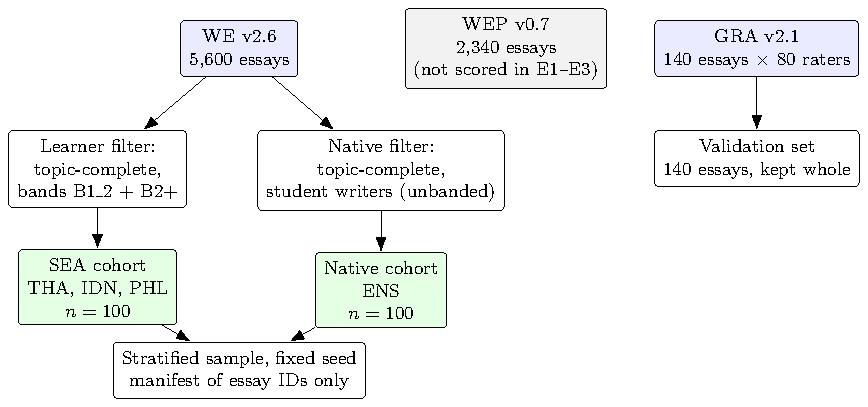
\includegraphics[width=0.8\textwidth]{figures/fig-sampling-flow}
\caption[Cohort construction and sampling flow]{Cohort construction
and sampling. Essay texts remain within licensed storage; the
reproducibility manifest records essay identifiers only.}
\label{fig:sampling-flow}
\end{figure}

\subsection*{Scoring target and ground truth}
Agents score each essay on the rubric's band scale; agreement with
ground truth is computed against the corpus's proficiency bands for
the main cohorts and against the GRA's multi-rater consensus for the
validation set. Inspection of the downloaded GRA archive (v2.1)
confirms its structure: each of the 140 essays carries ratings from
80 raters of varied L1 backgrounds, each scoring ten analytic
dimensions (0--10) grouped as Language, Content, and Attitude, plus a
holistic score out of 100. Per-essay rating dispersion across the 80
raters provides the human-disagreement benchmark against which BDS is
compared. Two properties of the archive shape the E3 design. First,
all 140 rated essays address the part-time-job prompt, so the
validation set is single-topic. Second, the raters disagree
substantially among themselves (mean within-essay standard deviation
of the Content ratings $\approx 1.8$ on the 0--10 scale):
disagreement among evaluators, human or artificial, is the normal
condition of essay assessment, and the question E3 asks is whether
the panel's divergence tracks the essays on which \emph{humans}
diverge.

\subsection*{Licence and handling}
ICNALE is distributed free for research; its terms of use prohibit
redistribution of any part of the data, and the project's required
citation is the ICNALE Guide \citep{ishikawa2023icnale}. In this
project, essay texts are stored only in access-controlled university
storage, never committed to version control, and no essay text is
reproduced in this thesis beyond short quotation where the licence
permits; the reproducibility package releases code, prompts,
configurations, and essay-ID manifests only. The data are
de-identified by the distributor, and their use falls under the
ethics exemption described in Section~\ref{sec:ethics}.

\section{Experimental Design}
\label{sec:experimental-design}

Three experiments test the four hypotheses
(Table~\ref{tab:experiments}). All conditions share the same
determinism guarantees: temperature fixed at $0.0$, structured JSON
outputs, exact model versions pinned in the experiment configuration,
and a fixed random seed for all sampling, so that every result in
Chapter~4 is reproducible from the released configuration, prompts,
and essay-identifier manifest.

\begin{table}[htbp]
\centering
\caption[Overview of Experiments E1--E3]{Overview of the three
experiments: data, conditions, and the hypotheses each tests.}
\label{tab:experiments}
\small
\begin{tabular}{p{1.2cm} p{3.4cm} p{4.3cm} p{2.2cm}}
\hline
Exp. & Data & Conditions & Tests \\
\hline
E1 & SEA + native cohorts ($n \approx 100$ each) & Single-agent
baseline vs.\ CAMPS $k{=}3$, four models & H1; H2 (part) \\[3pt]
E2 & Same cohorts & CAMPS $k{=}5$ with and without meta-adjudicator;
consensus-weight sweep ($\Delta w = 0.05$); ablation over
$k \in \{1,3,5\}$ & H2; H4 \\[3pt]
E3 & GRA validation set (140 essays $\times$ 80 raters) & CAMPS
$k{=}5$; ROC calibration of $\tau$ on a calibration split, evaluation
on a hold-out split & H3 \\
\hline
\end{tabular}
\end{table}

\textbf{Experiment E1 (scaled replication)} scores both cohorts under
the single-agent baseline and the pilot's three-agent panel on all
four models, establishing whether the gap exists at scale (H1) and
providing the $k{=}3$ reference for E2.

\textbf{Experiment E2 (extended architecture)} scores the same essays
under the five-agent panel, with and without the meta-adjudicator,
and sweeps the consensus weights in steps of $0.05$ under
$\sum_i w_i = 1$, tracing the fairness--accuracy frontier from which
H4's boundary is read off empirically. The ablation over $k$
separates the contribution of panel size from that of the
adjudicator.

\textbf{Experiment E3 (detection validation)} computes BDS for the
140 GRA essays. Human rating dispersion provides the reference notion
of a genuinely contested essay; the threshold $\tau$ is calibrated on
a random half of the GRA set (Youden's $J$) and evaluated on the
held-out half, reporting sensitivity, false-positive rate, and area
under the ROC curve.

\section{Alternatives Considered}
\label{sec:alternatives}

The rubric of this thesis requires critical awareness of alternatives;
this section records the designs considered and rejected, and why.

\emph{Training-time cultural adaptation}, as in CultureLLM
\citep{li2024culturellm}, fine-tunes models on culturally augmented
data. It is rejected on deployment grounds: it requires weight access
or fine-tuning budgets unavailable to most educational institutions,
must be repeated for every model generation, and cannot be audited by
the deploying institution. \emph{Activation steering}, as in FairSteer
\citep{li2025fairsteer}, intervenes on internal representations and is
infeasible for API-only access by construction
(Section~\ref{sec:lit-debias}).

\emph{Single-prompt debiasing}, instructing one evaluator to ``score
fairly across cultures'', was considered and rejected for two reasons:
it collapses the plurality of standards back into a single opaque
judgment, so cultural bias cannot be measured, only asserted away; and
it provides no divergence signal, so there is nothing to calibrate a
human-review trigger against. The single-agent baseline in E1
approximates this design and provides its empirical comparison.

\emph{Inter-agent debate}, as in MACD \citep{tan2026macd}, lets agents
deliberate before judgment. For evaluative scoring this is rejected on
two grounds: the MALIBU results \citep{mirza2025malibu} show that
agent interaction can amplify bias, and deliberation before scoring
destroys the independence that makes the Bias Divergence Score
meaningful. CAMPS instead confines deliberation to the optional
meta-adjudicator, which operates after independent scores are
recorded.

\emph{Recruiting external human raters} for validation was rejected on
ethics-scope and timeline grounds (Section~\ref{sec:ethics}); the GRA
archive supplies eighty raters per essay without new data collection.
Alternative corpora were considered and eliminated on design grounds
in Section~\ref{sec:data}.

\section{Ethical Considerations}
\label{sec:ethics}

This research analyses de-identified secondary data only and is
covered by an RMIT human research ethics exemption (Project ID 31036).
The ICNALE corpus is distributed for research with all personal
identifiers removed by the distributor; no attempt is made to
re-identify any writer, no essay text is redistributed or committed to
version control, and storage follows the project's research data
management plan (university-managed storage, access restricted to the
research team). Validation re-scoring is performed by the research
team only; no external participants are recruited, and any future
extension involving human participants would require a new ethics
assessment before commencing.

Two further considerations shape the design rather than merely
constrain it. First, cultural essentialism: scoring agents are
calibrated to \emph{documented rhetorical traditions}, not to
nationalities, and L1 cohorts are treated throughout as proxies for
rhetorical tradition rather than identity
(Section~\ref{sec:lit-rhetoric}). Second, downstream welfare: CAMPS is
designed as a human-in-the-loop system precisely because the cost of a
misclassified essay falls on a student; the BDS mechanism exists to
route uncertain judgments to a human rather than automate them. The
use of generative AI tools in this project is disclosed in accordance
with course policy.

\section{Metrics and Statistical Protocol}
\label{sec:metrics}

\textbf{Primary metric.} The primary fairness quantity is the
\emph{cohort score gap}: the difference in mean panel score between
the native and Southeast Asian cohorts,
\begin{equation}
\Delta = \overline{S^{*}}_{\mathrm{native}}
        - \overline{S^{*}}_{\mathrm{SEA}},
\end{equation}
computed on proficiency-matched cohorts so that, absent bias, the
expected gap is near zero. This operationalisation follows the pilot
and is forced by a property of the reference data: the native cohort
writes as an unbanded reference group (ICNALE assigns CEFR bands to
learners only), so band-agreement statistics are undefined for it.
Agreement with graded ground truth is reported secondarily where such
truth exists: Quadratic Weighted Kappa,
\begin{equation}
\kappa_w = 1 - \frac{\sum_{i,j} w_{ij} O_{ij}}
                     {\sum_{i,j} w_{ij} E_{ij}},
\qquad w_{ij} = \frac{(i-j)^2}{(R-1)^2},
\end{equation}
against proficiency bands for the learner cohorts, and against the
multi-rater human consensus for the GRA validation set (E3).

\textbf{Uncertainty.} Every reported statistic carries its $n$, and
every proportion or $\kappa_w$ is reported with a 95\% percentile
bootstrap confidence interval (10{,}000 resamples, fixed seed).
Following the statistical-reporting guidance adopted for this thesis,
confidence intervals are the primary inferential device;
$p$-values are reported only for the pre-registered hypothesis tests
(Fisher's $z$ on cohort correlation differences for H1), and no
post-hoc significance testing is performed on exploratory findings.

\textbf{Detection metrics.} BDS performance in E3 is reported as
sensitivity, false-positive rate, and area under the ROC curve on the
held-out split, with the calibrated threshold $\tau$ stated
explicitly.

\textbf{Weight calibration.} The E2 weight sweep reports the full
frontier rather than a single optimum: at each weight vector, the
cohort score gap (fairness) and $\kappa_w$ against CEFR bands on the
banded learner cohort (accuracy; the native reference is unbanded)
are recorded, and the H4 boundary is read off the resulting Pareto
frontier.

\textbf{Reproducibility.} All tables and figures in Chapter~4 are
generated by the analysis scripts in the project repository from the
logged scoring calls; no statistic is computed by hand. The
configuration file, prompts, essay-identifier manifest, and analysis
code are released; essay texts are not (Section~\ref{sec:data}).
